\documentclass[11pt]{article}
\usepackage{graphicx}
\usepackage{booktabs}
\usepackage{amsmath}
\usepackage{url}
\begin{document}
\sloppy
\title{Transcriptional Metabolic-State Clustering}
\author{}
\date{}
\maketitle

\section{Methods}
The analysis used 58,843 cells globally and 3,624 cells in the exact \texttt{cell\_subtype=CD8 T cells} subset. Both cores used the user-supplied feature set \texttt{inputs/metabolic\_genes\_total.csv}; its SHA-256 is recorded in the analysis manifest and both core results. The global and CD8 analyses retained 1,646 and 1,318 metabolic genes after prevalence filtering, respectively. Feature scaling was Scanpy scale(zero\_center=False, max\_value=10). The seed grid was 0, 17, 42, 73, 101.

Per-cell library-size normalization to 10,000 followed by log1p was
\begin{equation}
\label{eq:normalization}
x'_{ig}=\log\!\left(1+\frac{10^4 x_{ig}}{\sum_g x_{ig}}\right).
\end{equation}
Equation~\ref{eq:normalization} defines normalization, where $x_{ig}$ is the raw count for gene $g$ in cell $i$, $\sum_g x_{ig}$ is the all-feature library-size denominator for cell $i$, and $x'_{ig}$ is normalized expression.

\section{Question 1: Global metabolic partitions}
Candidate partitions were observed, but distinct biological metabolic states remain inconclusive. At resolution 0.4, the global core produced 13 clusters ranging from 1,051 to 9,041 cells. Its silhouette, Calinski--Harabasz, Davies--Bouldin, mean pairwise ARI, and minimum pairwise ARI were 0.218, 7268.856, 1.484, 0.951, and 0.919, respectively. 5 of 19 random controls equaled or exceeded the matched-$k$ metabolic silhouette; the descriptive add-one rank fraction was 0.3.

Figure~\ref{fig:global_umap} shows the global embedding, and Figure~\ref{fig:global_diagnostics} shows its diagnostics.
\begin{figure}[h]
\centering
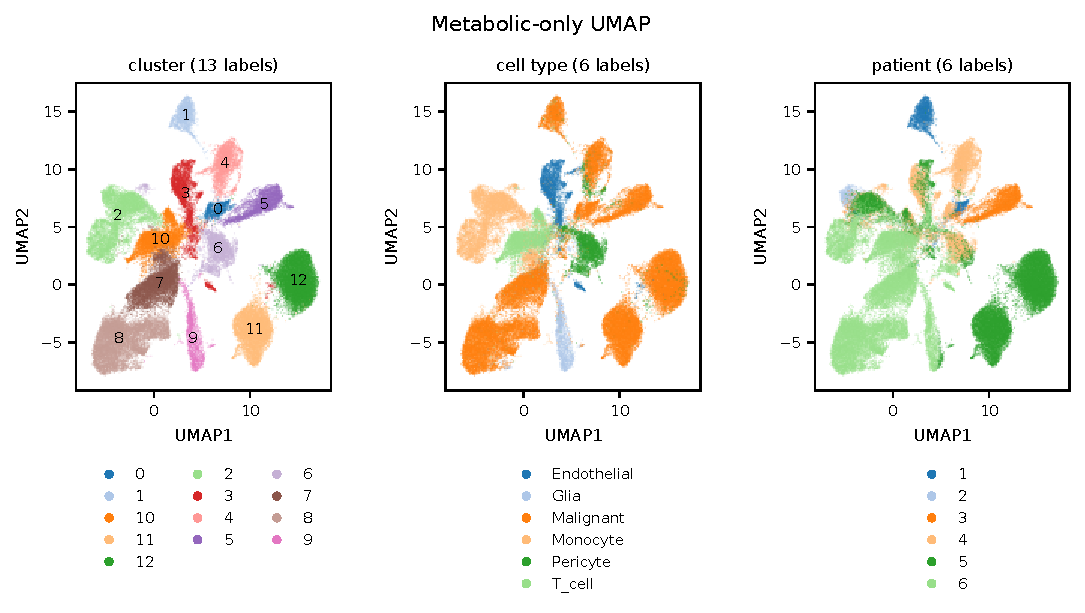
\includegraphics[width=0.95\linewidth,height=0.78\textheight,keepaspectratio]{../figures/metabolic_umap.pdf}
\caption{Global metabolic-gene UMAP colored by the saved cluster labels.}
\label{fig:global_umap}
\end{figure}
\begin{figure}[h]
\centering
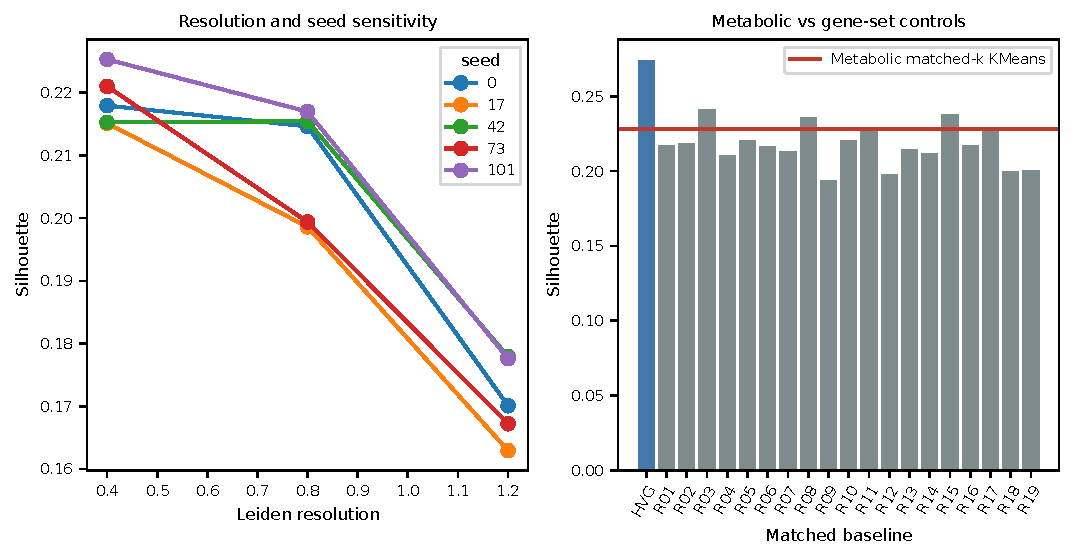
\includegraphics[width=0.95\linewidth,height=0.78\textheight,keepaspectratio]{../figures/clustering_diagnostics.pdf}
\caption{Global resolution, stability, and control diagnostics.}
\label{fig:global_diagnostics}
\end{figure}

\section{Question 2: Descriptive group associations}
Associations with recorded groups are descriptive and non-causal. Global patient, cell-type, and cell-subtype NMI values were 0.521, 0.508, and 0.656. Across patient-specific sensitivity analyses, global-versus-within ARI ranged from 0.117 to 0.942; the weakest patient was patient 3 with 3,287 cells. These values do not establish independence, mechanism, or causal separation.

Table~\ref{tab:clustering_metrics} summarizes the two saved cores.
\begin{table}[h]
\centering
\caption{Saved clustering metrics for the global and CD8 cores}
\label{tab:clustering_metrics}
\begin{tabular}{lrr}
\toprule
Metric & Global & CD8 T cells \\
\midrule
Silhouette & 0.218 & 0.093 \\
Calinski--Harabasz & 7268.856 & 399.641 \\
Davies--Bouldin & 1.484 & 2.205 \\
Mean pairwise ARI & 0.951 & 0.736 \\
Minimum pairwise ARI & 0.919 & 0.583 \\
Clusters & 13 & 6 \\
\bottomrule
\end{tabular}
\end{table}

\section{Question 3: CD8 T-cell subset}
Candidate partitions were observed in CD8 T cells, but distinct biological metabolic states remain inconclusive. At resolution 0.4, the CD8 core produced 6 clusters ranging from 55 to 1,872 cells. 17 of 19 random controls equaled or exceeded the matched-$k$ metabolic silhouette; the descriptive add-one rank fraction was 0.9. Across patient-specific sensitivity analyses, global-versus-within ARI ranged from 0.486 to 0.832; the weakest patient was patient 6 with 2,776 cells.

Figure~\ref{fig:cd8_umap} shows the CD8 embedding, and Figure~\ref{fig:cd8_diagnostics} shows its diagnostics.
\begin{figure}[h]
\centering
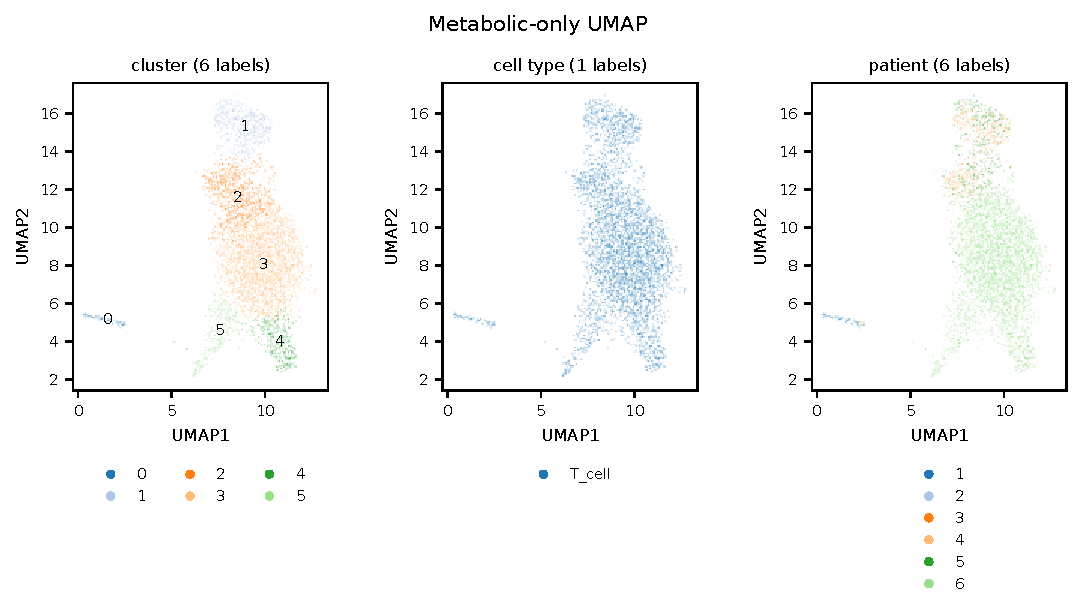
\includegraphics[width=0.95\linewidth,height=0.78\textheight,keepaspectratio]{../figures/cd8_analysis/metabolic_umap.pdf}
\caption{CD8 T-cell metabolic-gene UMAP colored by the saved cluster labels.}
\label{fig:cd8_umap}
\end{figure}
\begin{figure}[h]
\centering
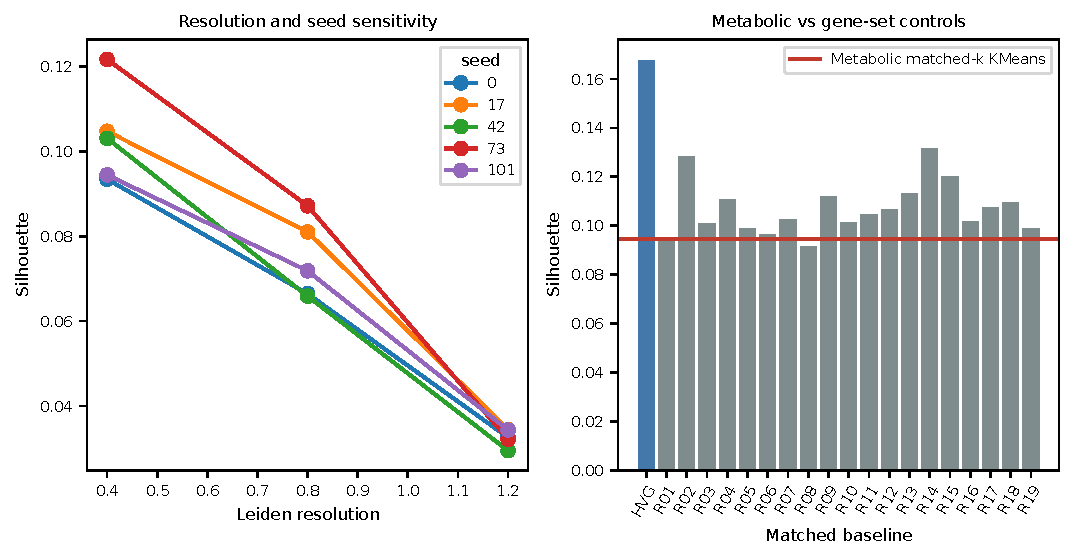
\includegraphics[width=0.95\linewidth,height=0.78\textheight,keepaspectratio]{../figures/cd8_analysis/clustering_diagnostics.pdf}
\caption{CD8 T-cell resolution, stability, and control diagnostics.}
\label{fig:cd8_diagnostics}
\end{figure}

\section{Resolution selection and limits}
Resolution selection maximized median silhouette among candidates passing the mean pairwise ARI stability filter; mean pairwise ARI was the tie-breaker. The random-control ranks are descriptive benchmarks, not biological P values. Resolution selection and cluster assessment used the same dataset, and patient-level sensitivity is not held-out validation. The results therefore support exploratory computational partitions only.

\section{Verified literature}
\begin{itemize}
\item \url{https://doi.org/10.1038/s41588-022-01061-8}
\item \url{https://doi.org/10.1186/s13059-017-1382-0}
\end{itemize}
\end{document}
